\newpage
\newpage
\section{Description of the final product}
The final project is hosted at \href{https://code-quality-honours.herokuapp.com/}{https://code-quality-honours.herokuapp.com/} See Appendix U.
\newline
\textbf{Overall Product}
\newline
In Figure \RefFig{fig:finalproduct} we can see a screenshot of the final product, the code editor on the left and the analysis output on the right.
\begin{figure}[h]
    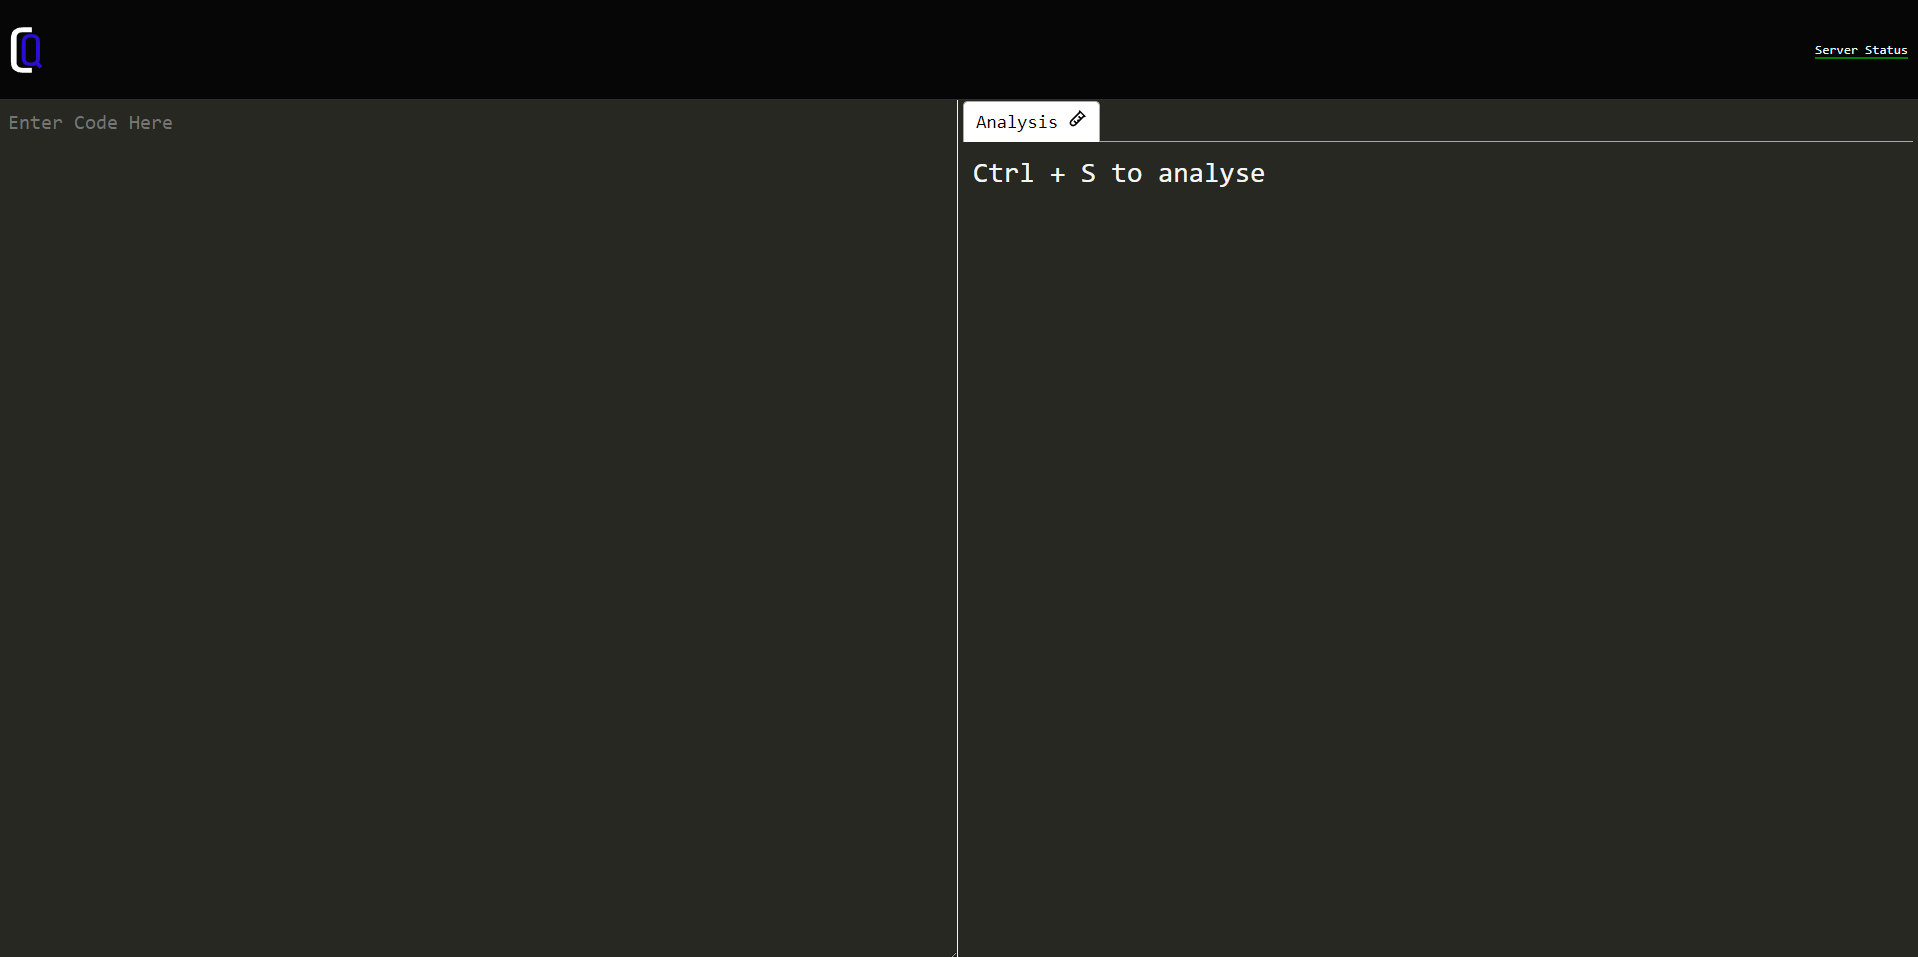
\includegraphics[width=.5\textwidth]{images/final-screenshot.png}
    \caption{Final Product See Appendix U}
    \Description{Final Product See Appendix U}
    \label{fig:finalproduct}
\end{figure}
\newline
\newline
\textbf{Code Editor}
\newline
In Figure \RefFig{fig:autocomplete} we can see a screenshot of the autocomplete feature, this allows the user to autocomplete code using a list of all 
the javascript reserved words and any words already typed in the editor by pressing tab
\newline
The user will also have brackets and strings autofilled while typing.
\begin{figure}[h]
    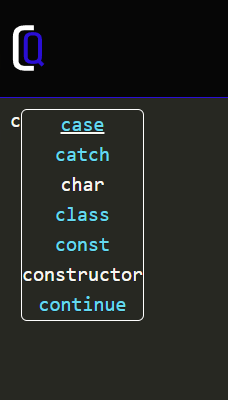
\includegraphics[width=.3\textwidth]{images/autocomplete.png}
    \caption{AutoComplete See Appendix U}
    \Description{AutoComplete See Appendix U}
    \label{fig:autocomplete}
\end{figure}
In Figure \RefFig{fig:Highliting} we can see the code the user has entered that has been highlighted.
\begin{figure}[h]
    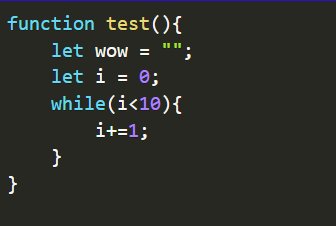
\includegraphics[width=.3\textwidth]{images/Highlighted.png}
    \caption{Highlighted Source Code See Appendix U}
    \Description{Highlighted Source Code See Appendix U}
    \label{fig:Highliting}
\end{figure}
\newline
\newline
\textbf{Analysis}
\newline
In Figure \RefFig{fig:output} we can see the output in the analysis panel, this displays the output of the analysis on the code alongside the 
source code. Also in Figure \RefFig{fig:clickfunc} we can see that clicking on a element in the output panel highlights that code within the code editor. Finally in Figure \
The download button shown in \RefFig{fig:downloadbutton} allows the user to download a copy of the report.
\newline
In Figure \RefFig{fig:astpanel} we can see the ast panel which allows users to view the AST of their source code.
\begin{figure}[h]
    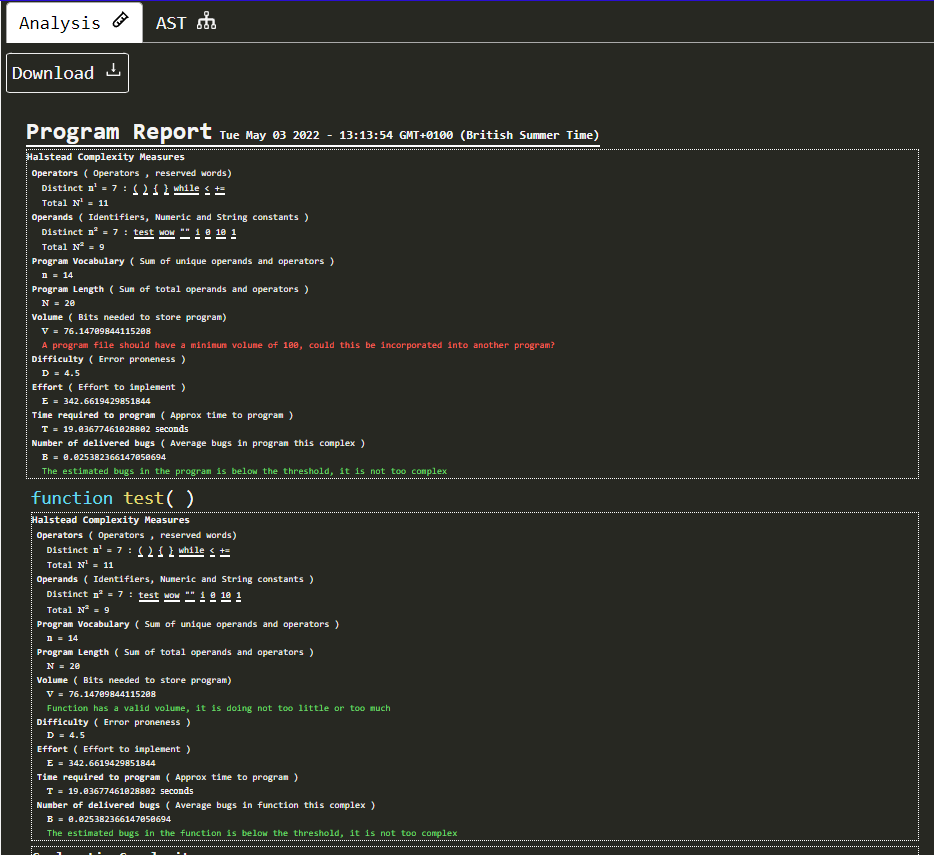
\includegraphics[width=.5\textwidth]{images/analysisoutput.png}
    \caption{Analysis Output See Appendix U}
    \Description{Analysis Output See Appendix U}
    \label{fig:output}
\end{figure}

\begin{figure}[h]
    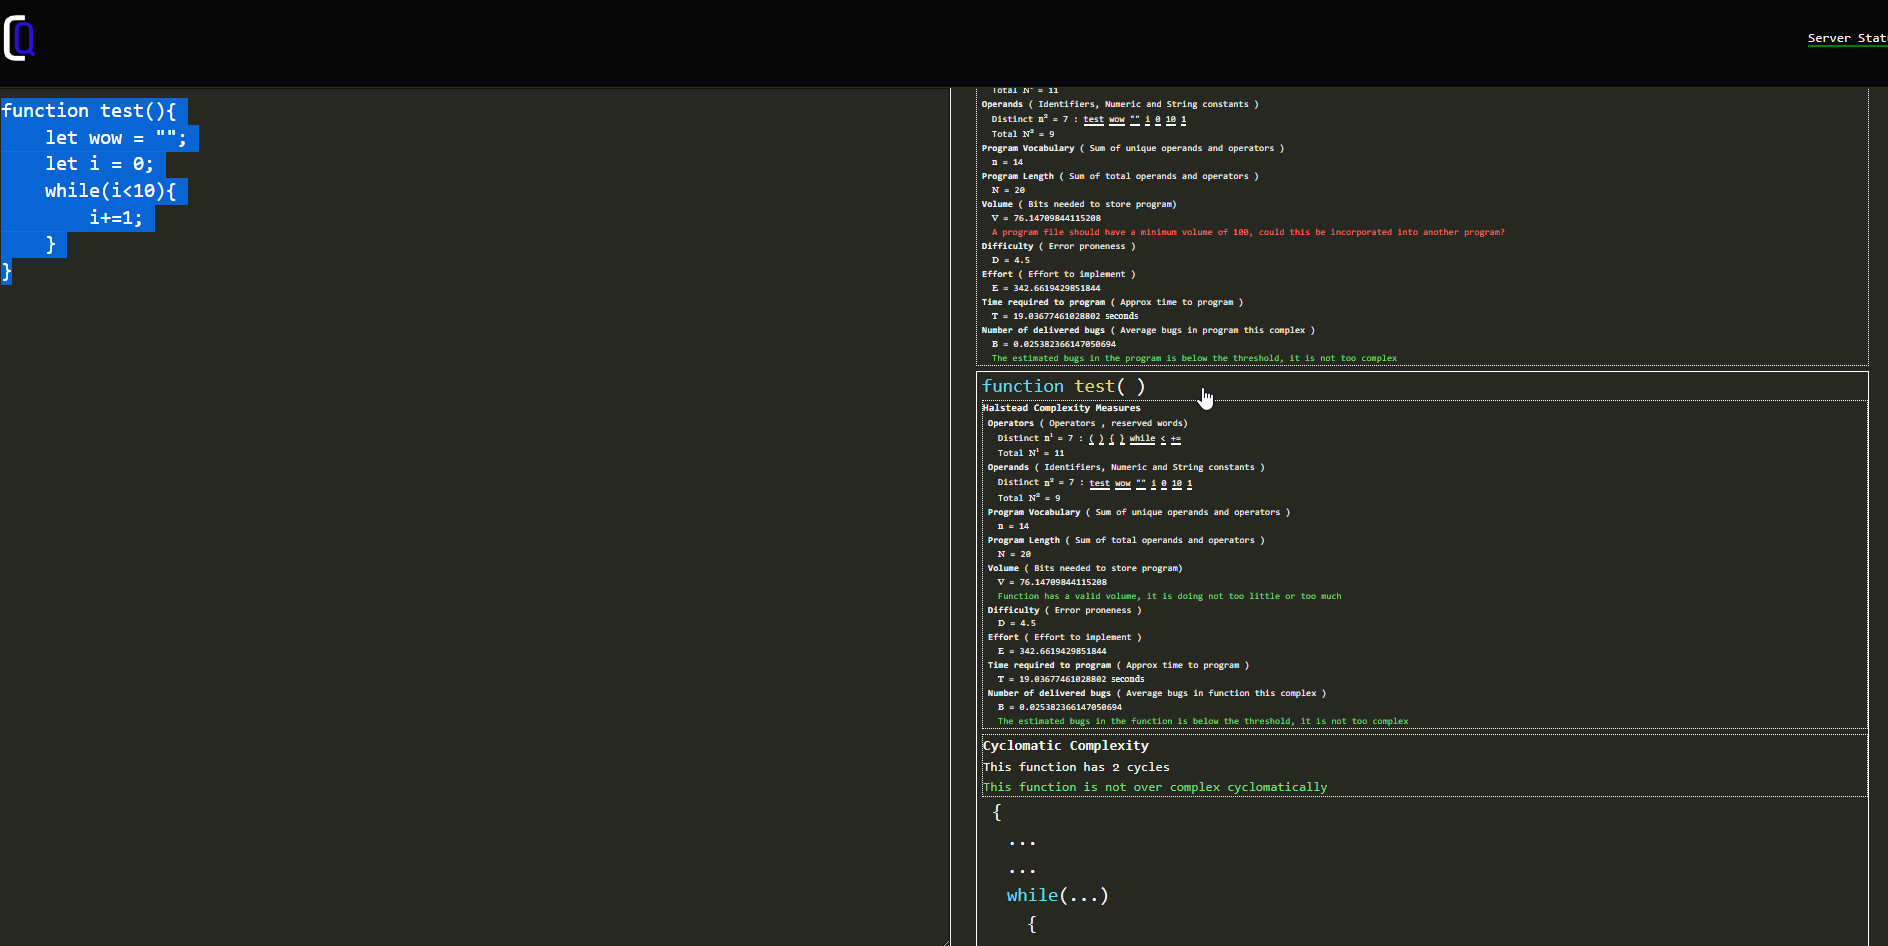
\includegraphics[width=.5\textwidth]{images/clickfunc.png}
    \caption{Clicking on function in analysis See Appendix U}
    \Description{Clicking on function in analysis See Appendix U}
    \label{fig:clickfunc}
\end{figure}
\begin{figure}[h]
    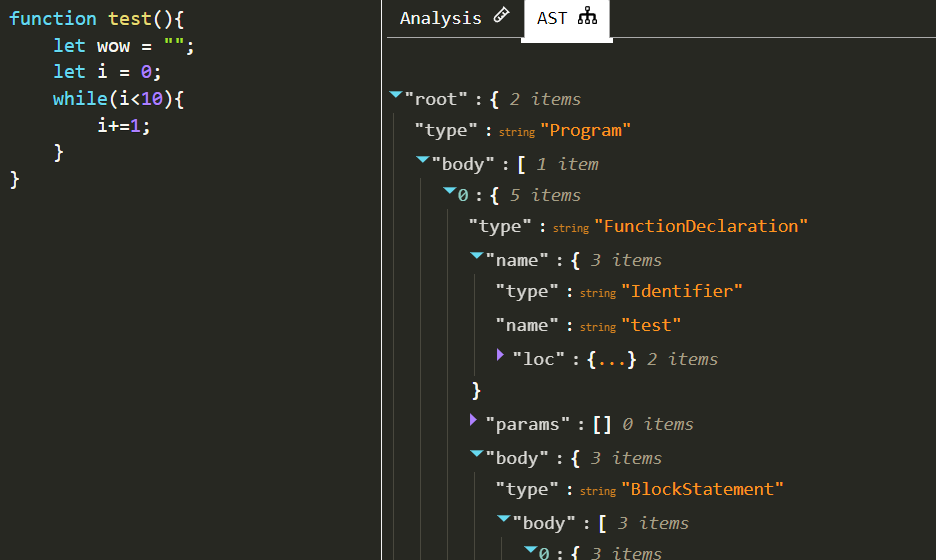
\includegraphics[width=.5\textwidth]{images/ast.png}
    \caption{AST panel See Appendix U}
    \Description{AST panel See Appendix U}
    \label{fig:astpanel}
\end{figure}
\begin{figure}[h]
    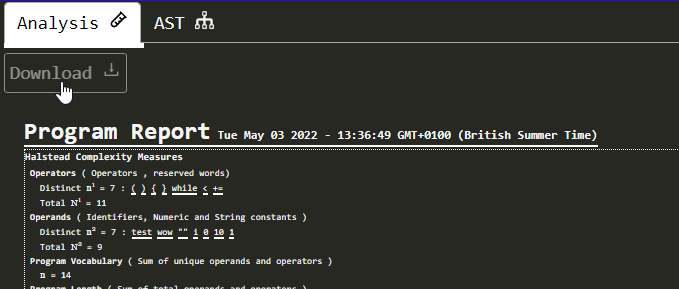
\includegraphics[width=.4\textwidth]{images/downloadbutton.png}
    \caption{Download Button See Appendix U}
    \Description{Download Button See Appendix U}
    \label{fig:downloadbutton}
\end{figure}

In figure \RefFig{fig:syntax1} we can see that the user has entered incorrect syntax. By then opening the syntax panel and clicking on the error , 
the user can find the syntax error in the code, as shown in Figure \RefFig{fig:syntax2}
\begin{figure}[h]
    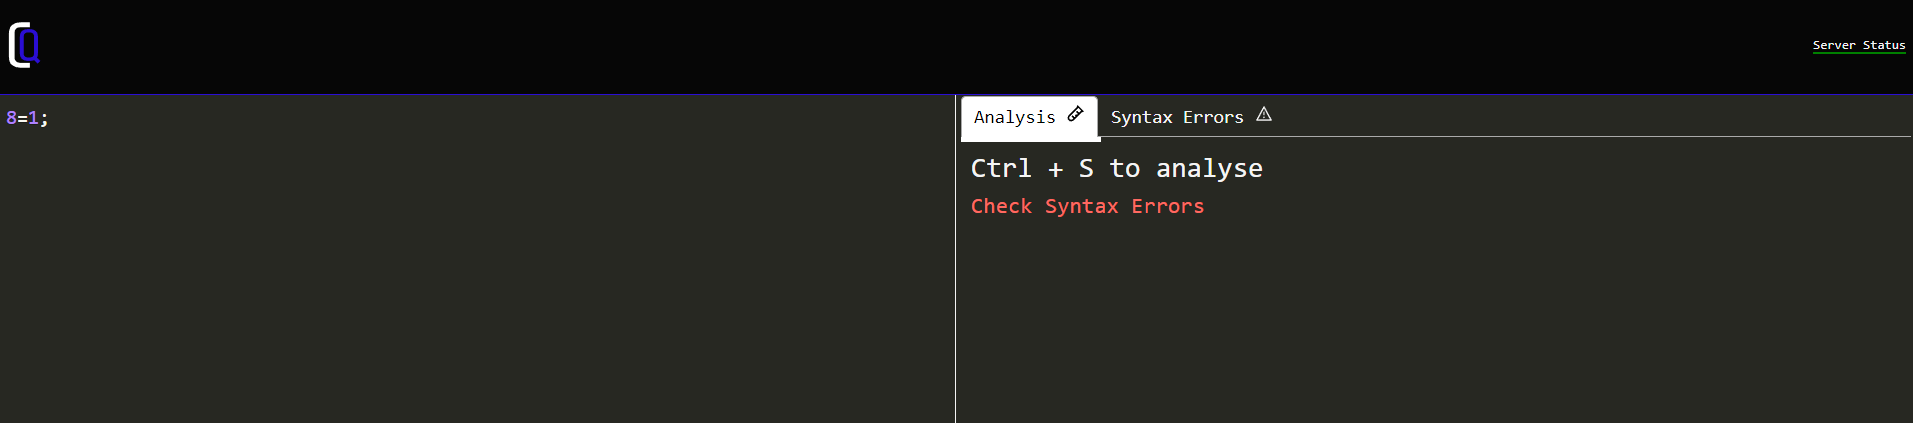
\includegraphics[width=.5\textwidth]{images/syntax1.png}
    \caption{Syntax Error See Appendix U}
    \Description{Syntax Error See Appendix U}
    \label{fig:syntax1}
\end{figure}
\begin{figure}[h]
    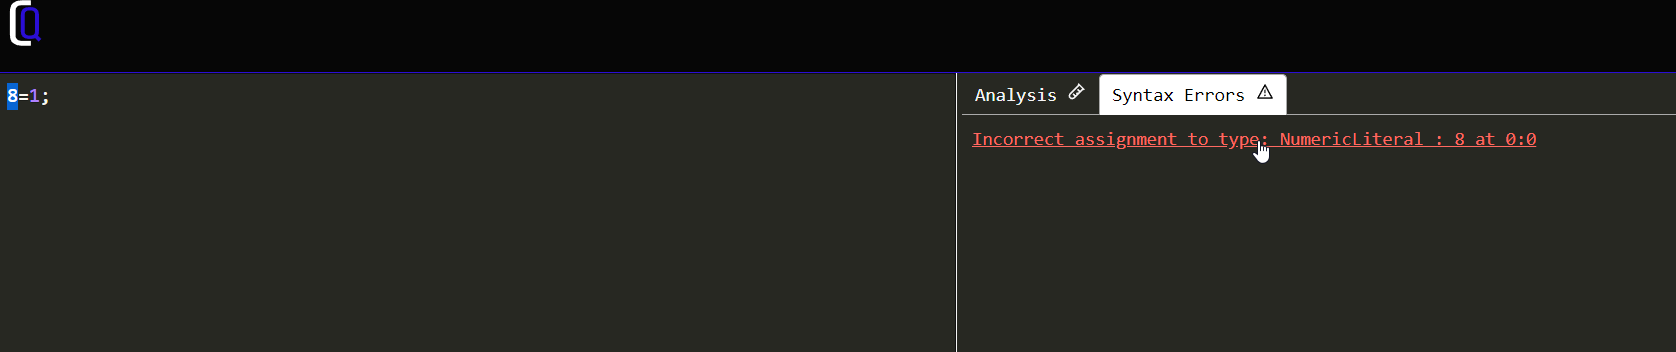
\includegraphics[width=.5\textwidth]{images/syntax2.png}
    \caption{Syntax Error Clicking See Appendix U}
    \Description{Syntax Error Clicking See Appendix U}
    \label{fig:syntax2}
\end{figure}
\newpage